%% BioMed_Central_Tex_Template_v1.06
%%                                      %
%  bmc_article.tex            ver: 1.06 %
%                                       %

%%IMPORTANT: do not delete the first line of this template
%%It must be present to enable the BMC Submission system to
%%recognise this template!!

%%%%%%%%%%%%%%%%%%%%%%%%%%%%%%%%%%%%%%%%%
%%                                     %%
%%  LaTeX template for BioMed Central  %%
%%     journal article submissions     %%
%%                                     %%
%%          <8 June 2012>              %%
%%                                     %%
%%                                     %%
%%%%%%%%%%%%%%%%%%%%%%%%%%%%%%%%%%%%%%%%%

%%%%%%%%%%%%%%%%%%%%%%%%%%%%%%%%%%%%%%%%%%%%%%%%%%%%%%%%%%%%%%%%%%%%%
%%                                                                 %%
%% For instructions on how to fill out this Tex template           %%
%% document please refer to Readme.html and the instructions for   %%
%% authors page on the biomed central website                      %%
%% https://www.biomedcentral.com/getpublished                      %%
%%                                                                 %%
%% Please do not use \input{...} to include other tex files.       %%
%% Submit your LaTeX manuscript as one .tex document.              %%
%%                                                                 %%
%% All additional figures and files should be attached             %%
%% separately and not embedded in the \TeX\ document itself.       %%
%%                                                                 %%
%% BioMed Central currently use the MikTex distribution of         %%
%% TeX for Windows) of TeX and LaTeX.  This is available from      %%
%% https://miktex.org/                                             %%
%%                                                                 %%
%%%%%%%%%%%%%%%%%%%%%%%%%%%%%%%%%%%%%%%%%%%%%%%%%%%%%%%%%%%%%%%%%%%%%

%%% additional documentclass options:
%  [doublespacing]
%  [linenumbers]   - put the line numbers on margins

%%% loading packages, author definitions

%\documentclass[twocolumn]{bmcart}% uncomment this for twocolumn layout and comment line below
\documentclass{bmcart}

%%% Load packages
\usepackage{amsthm,amsmath}
\usepackage{subcaption}
%\RequirePackage[numbers]{natbib}
%\RequirePackage[authoryear]{natbib}% uncomment this for author-year bibliography
%\RequirePackage{hyperref}
\usepackage[utf8]{inputenc} %unicode support
%\usepackage[applemac]{inputenc} %applemac support if unicode package fails
%\usepackage[latin1]{inputenc} %UNIX support if unicode package fails
\usepackage{graphicx}       % graphics
\usepackage{lmodern}

\graphicspath{ {../media/} }

%%%%%%%%%%%%%%%%%%%%%%%%%%%%%%%%%%%%%%%%%%%%%%%%%
%%                                             %%
%%  If you wish to display your graphics for   %%
%%  your own use using includegraphic or       %%
%%  includegraphics, then comment out the      %%
%%  following two lines of code.               %%
%%  NB: These line *must* be included when     %%
%%  submitting to BMC.                         %%
%%  All figure files must be submitted as      %%
%%  separate graphics through the BMC          %%
%%  submission process, not included in the    %%
%%  submitted article.                         %%
%%                                             %%
%%%%%%%%%%%%%%%%%%%%%%%%%%%%%%%%%%%%%%%%%%%%%%%%%

% \def\includegraphic{}
% \def\includegraphics{}

%%% Put your definitions there:
\startlocaldefs
\endlocaldefs

%%% Begin ...
\begin{document}

%%% Start of article front matter
\begin{frontmatter}

\begin{fmbox}
\dochead{Research}

%%%%%%%%%%%%%%%%%%%%%%%%%%%%%%%%%%%%%%%%%%%%%%
%%                                          %%
%% Enter the title of your article here     %%
%%                                          %%
%%%%%%%%%%%%%%%%%%%%%%%%%%%%%%%%%%%%%%%%%%%%%%

\title{ColabSurgVR: a virtual reality surgical planning and collaborative platform}

%%%%%%%%%%%%%%%%%%%%%%%%%%%%%%%%%%%%%%%%%%%%%%
%%                                          %%
%% Enter the authors here                   %%
%%                                          %%
%% Specify information, if available,       %%
%% in the form:                             %%
%%   <key>={<id1>,<id2>}                    %%
%%   <key>=                                 %%
%% Comment or delete the keys which are     %%
%% not used. Repeat \author command as much %%
%% as required.                             %%
%%                                          %%
%%%%%%%%%%%%%%%%%%%%%%%%%%%%%%%%%%%%%%%%%%%%%%

\author[
  addressref={aff1, aff2},                   % id's of addresses, e.g. {aff1,aff2}
  % corref={aff1},                       % id of corresponding address, if any
  % noteref={n1},                        % id's of article notes, if any
  email={b07401012@ntu.edu.tw}   % email address
]{\inits{Y.C.L}\fnm{Yi-Ching} \snm{Lee}}
\author[
  addressref={aff3},                   % id's of addresses, e.g. {aff1,aff2}
  corref={aff1},                       % id of corresponding address, if any
  % noteref={n1},                        % id's of article notes, if any
  email={b07401012@ntu.edu.tw}   % email address
]{\inits{Y.S.C.}\fnm{Yang-Sheng} \snm{Chen}}
\author[
  addressref={aff1, aff2},                   % id's of addresses, e.g. {aff1,aff2}
  % corref={aff1},                       % id of corresponding address, if any
  % noteref={n1},                        % id's of article notes, if any
  email={b07401012@ntu.edu.tw}   % email address
]{\inits{X.H.C}\fnm{Xu-Heng} \snm{Chiang}}
\author[
  addressref={aff1, aff4},                   % id's of addresses, e.g. {aff1,aff2}
  % corref={aff1},                       % id of corresponding address, if any
  % noteref={n1},                        % id's of article notes, if any
  email={b07401012@ntu.edu.tw}   % email address
]{\inits{J.S.C}\fnm{Jin-Shing} \snm{Chen}}
\author[
  addressref={aff3},                   % id's of addresses, e.g. {aff1,aff2}
  % corref={aff1},                       % id of corresponding address, if any
  % noteref={n1},                        % id's of article notes, if any
  email={b07401012@ntu.edu.tw}   % email address
]{\inits{Y.P.H}\fnm{Yi-Ping} \snm{Hung}}
%%%%%%%%%%%%%%%%%%%%%%%%%%%%%%%%%%%%%%%%%%%%%%
%%                                          %%
%% Enter the authors' addresses here        %%
%%                                          %%
%% Repeat \address commands as much as      %%
%% required.                                %%
%%                                          %%
%%%%%%%%%%%%%%%%%%%%%%%%%%%%%%%%%%%%%%%%%%%%%%

\address[id=aff1]{%                           % unique id
  \orgdiv{Department of Surgery},             % department, if any
  \orgname{National Taiwan University Hospital and National Taiwan University College of Medicine},          % university, etc
  \city{Taipei},                              % city
  \cny{Taiwan}                                    % country
}
\address[id=aff2]{%                           % unique id
  \orgdiv{Department of Medical Education},             % department, if any
  \orgname{National Taiwan University Hospital and National Taiwan University College of Medicine},          % university, etc
  \city{Taipei},                              % city
  \cny{Taiwan}                                    % country
}
\address[id=aff3]{%                           % unique id
  \orgdiv{Graduate Institute of Networking and Multimedia},             % department, if any
  \orgname{National Taiwan University},          % university, etc
  \city{Taipei},                              % city
  \cny{Taiwan}                                    % country
}
\address[id=aff4]{%                           % unique id
  \orgdiv{Department of Surgical Oncology},             % department, if any
  \orgname{National Taiwan University Cancer Center},          % university, etc
  \city{Taipei},                              % city
  \cny{Taiwan}                                    % country
}

% \address[id=aff2]{%
%   \orgdiv{Institute of Biology},
%   \orgname{National University of Sciences},
%   %\street{},
%   %\postcode{}
%   \city{Kiel},
%   \cny{Germany}
% }

%%%%%%%%%%%%%%%%%%%%%%%%%%%%%%%%%%%%%%%%%%%%%%
%%                                          %%
%% Enter short notes here                   %%
%%                                          %%
%% Short notes will be after addresses      %%
%% on first page.                           %%
%%                                          %%
%%%%%%%%%%%%%%%%%%%%%%%%%%%%%%%%%%%%%%%%%%%%%%

% \begin{artnotes}
% \note{Sample of title note}     % note to the article
% \note[id=n1]{Equal contributor} % note, connected to author
% \end{artnotes}

\end{fmbox}% comment this for two column layout

%%%%%%%%%%%%%%%%%%%%%%%%%%%%%%%%%%%%%%%%%%%%%%%
%%                                           %%
%% The Abstract begins here                  %%
%%                                           %%
%% Please refer to the Instructions for      %%
%% authors on https://www.biomedcentral.com/ %%
%% and include the section headings          %%
%% accordingly for your article type.        %%
%%                                           %%
%%%%%%%%%%%%%%%%%%%%%%%%%%%%%%%%%%%%%%%%%%%%%%%

\begin{abstractbox}

\begin{abstract} % abstract
% \parttitle{First part title} %if any
% Text for this section.

% \parttitle{Second part title} %if any
% Text for this section.
The integration of virtual reality (VR) in preoperative planning offers a transformative approach to complex surgeries. This study presents the development and application of a VR surgical planning system designed to enhance the accuracy and efficiency of preoperative planning through immersive, three-dimensional (3D) visualizations of patient-specific anatomy derived from 2D image data. Our system facilitates real-time, interactive collaboration among multidisciplinary teams, enabling a comprehensive evaluation of surgical strategies. The process involves semi-automatic segmentation and manual refinement to generate high-fidelity 3D models, optimized using mesh processing techniques. Initial validation through a pilot study with clinical participants demonstrated the system's functional accuracy and potential to improve surgical outcomes. This research highlights the significant advancements in surgical planning technology and outlines future directions for further enhancement and broader application.
\end{abstract}

%%%%%%%%%%%%%%%%%%%%%%%%%%%%%%%%%%%%%%%%%%%%%%
%%                                          %%
%% The keywords begin here                  %%
%%                                          %%
%% Put each keyword in separate \kwd{}.     %%
%%                                          %%
%%%%%%%%%%%%%%%%%%%%%%%%%%%%%%%%%%%%%%%%%%%%%%

\begin{keyword}
\kwd{Virtual Reality}
\kwd{Preoperative Planning}
\kwd{3D Visualization}
\kwd{Surgical Collaboration}
\end{keyword}

% MSC classifications codes, if any
%\begin{keyword}[class=AMS]
%\kwd[Primary ]{}
%\kwd{}
%\kwd[; secondary ]{}
%\end{keyword}

\end{abstractbox}
%
%\end{fmbox}% uncomment this for two column layout

\end{frontmatter}

%%%%%%%%%%%%%%%%%%%%%%%%%%%%%%%%%%%%%%%%%%%%%%%%
%%                                            %%
%% The Main Body begins here                  %%
%%                                            %%
%% Please refer to the instructions for       %%
%% authors on:                                %%
%% https://www.biomedcentral.com/getpublished %%
%% and include the section headings           %%
%% accordingly for your article type.         %%
%%                                            %%
%% See the Results and Discussion section     %%
%% for details on how to create sub-sections  %%
%%                                            %%
%% use \cite{...} to cite references          %%
%%  \cite{koon} and                           %%
%%  \cite{oreg,khar,zvai,xjon,schn,pond}      %%
%%                                            %%
%%%%%%%%%%%%%%%%%%%%%%%%%%%%%%%%%%%%%%%%%%%%%%%%

%%%%%%%%%%%%%%%%%%%%%%%%% start of article main body
% <put your article body there>

%%%%%%%%%%%%%%%%
%% Background %%
%%
\section{Introduction}
Planning for complex surgical procedures presents numerous challenges and difficulties, primarily due to the intricate and variable nature of human anatomy. The success of such interventions heavily relies on the surgeon's ability to anticipate and navigate these complexities, underscoring the importance of integration of advanced imaging and planning tools that can provide a detailed and accurate representation of the patient-specific anatomy \cite{RN30}.

Virtual reality (VR) offers a promising solution to the challenges inherent in complex surgery planning \cite{RN32, RN31, RN2, RN24}. By providing immersive, three-dimensional (3D) visualizations of patient-specific anatomy, VR enables surgeons to interact with and manipulate anatomical models in a immersive nature. This interactive capability allows for a more thorough visuospatial conversion from two-dimensional (2D) images, optimizing strategic planning. Supported by advancements in computing power and hardware \cite{RN33}, applications of VR in preoperative planning have demonstrated clinical benefits for both patients and physicians, including changes in preoperative planning \cite{RN17, RN13, RN37, RN10, RN44, RN29}, improvements in surgical decision-making \cite{RN5}, and reductions in operative times \cite{RN36, RN28} across multiple surgical subspecialties \cite{RN38, RN2}.

Integration with communication technologies can further enhance the convenience and accessibility of preoperative planning. The flexibility provided by enabling real-time interaction between multidisciplinary teams ensures that critical insights and decisions can be made without the need for all team members to be physically present in the same location \cite{RN26, RN6}. The combination of virtual reality with network communication can facilitate mutual understanding and collaboration among surgical team members, which is crucial for both patient outcomes and physician efficiency \cite{RN62, RN25}.

In this work, we develop a VR surgical planning system, ColabSurgVR. This system allows multiple users to examine the patient organ model reconstructed from computed tomography (CT) dataset and collaborate on forming a preoperative plan in real time. Also we describe a protocol to process patient-specific image datas into 3D models for immersive interaction in virtual environment. To test the use case and performance, we have conducted a pilot user study involving 10 physicians to examine real world patient data present the preliminary qualitative result.

\section{System Design and Implementation}
Our proposed pipeline takes the imaging data from CT and generates a 3D model for viewing in virtual reality. It involves processing steps to segment the content of the images and reconstrct the anatomy for the patient. The resultant 3D models will be further modified and then imported into our VR surgical planning system supporting immersive visulization and intuitive interaction. The user can assess the system either by extended reality or conventional devices. See Figure \ref{fig:Scheme} for schematic representation of our workflow and system architecture.



\begin{figure}
  \centering
  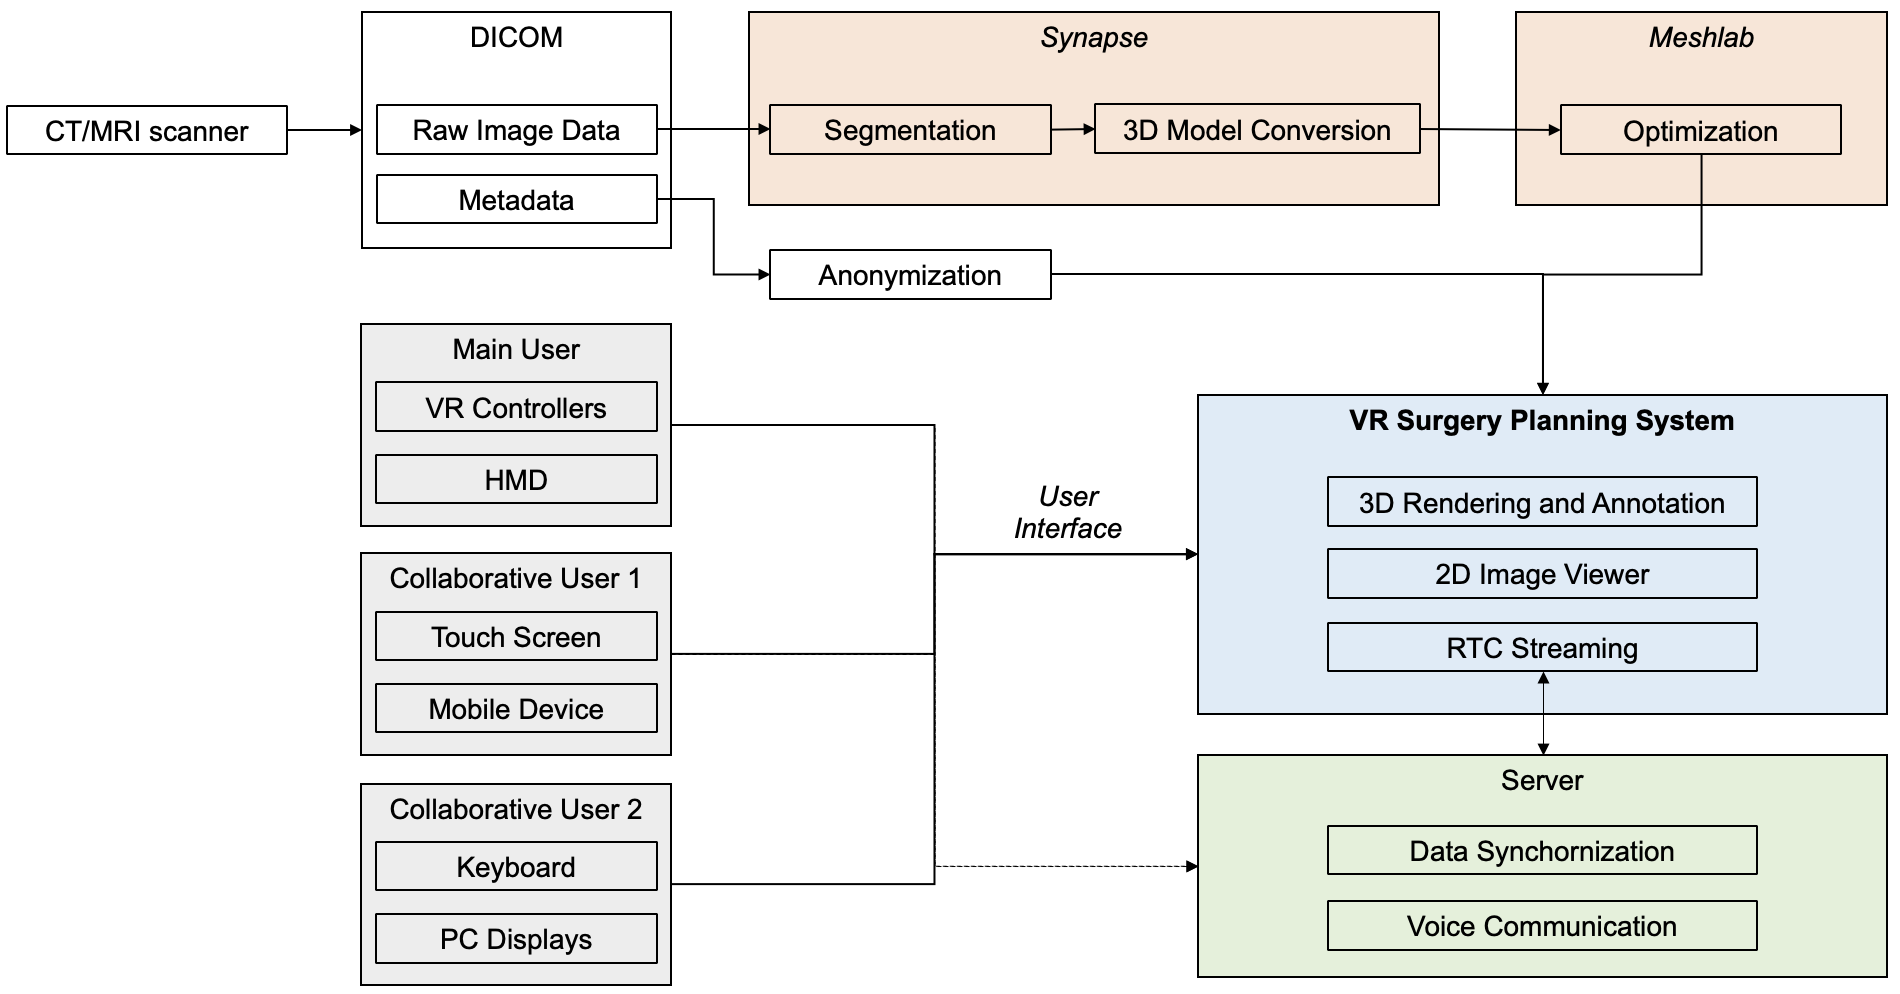
\includegraphics[width=.9\linewidth]{../Media/Scheme}  
  \caption{System architecture of ColabSurgVR.}
  \label{fig:Scheme}
\end{figure}

\subsection{Medical Image Acquisition}
Volumetric data acquired from computer tomography (CT) scanners was output in the Digital Imaging and Communication (DICOM) format. The slice thickness was set to 1 mm for acquisition protocol, and all images were reconstructed into 3 mm slices for subsequent interpretation and analysis.
\subsection{Segmentation and Virtual Reality Object Generation}
The DICOM images were anonymized and then imported into a commercially available medical imaging workstation, Synapse 3D (Fujifilm, Tokyo, Japan), for 3D visualization, segmentation, and 3D model generation. Skin, bones, vascular structures, bronchi, bronchopulmonary segments, and tumors (if present) were segmented from the CT datasets semiautomatically using built-in extraction functions in Synapse 3D Viewer and Lung Analysis Resection applications. Additional segmentation of small branches and border modification were performed manually by assigning or deleting pixels in the image dataset to the corresponding desired anatomic structures. Isolation of submodels (e.g., isolating a rib from the bone models) was also conducted by manually dividing the segmented data. During manual refinement, the CT image data with adjustable window settings and a 3D volumetric rendering of the segmented region were both available to the operator for optimal evaluation and stereoscopic visualization. After segmentation, texture mapping was applied to define surface texture and color information of the segmented data. The resulting data were then exported into a standard tessellation language (STL) file format.
\subsection{Model Optimization}
To optimize the mesh representation of the 3D models, an open-source 3D mesh processing software, MeshLab (version 2023.12), was utilized \cite{RN19}. The STL files were imported into MeshLab and first underwent a series of cleaning operations, including the removal of duplicated vertices, unreferenced vertices, and zero-area faces to enhance the mesh integrity. Then, quadric edge collapse decimation targeting a 50$\%$ reduction in face count was applied to reduce the polygon count while preserving essential geometric features \cite{RN20}. Laplacian smoothing was applied to ensure balanced surface smoothness. Normals were recomputed to correct any lighting and shading inconsistencies using weighted normal calculation. Finally, isolated mesh components were removed, with the minimum component size set to 10$\%$ of the overall model diameter. The optimized meshes were then exported in OBJ format for integration into our VR surgery planning system.
\subsection{VR Environment Development}
For the presentation and interaction with the 3D models, we developed our software using the Unity 3D engine (Unity Technologies, San Francisco, CA, version 2020.3) and integrated it with the Meta XR All-in-One SDK (version 60). We employed the Universal Rendering Pipeline (URP) from Unity, which facilitated optimized graphics performance across various platforms, including mobile devices, PCs, and head-mounted displays (HMDs) utilized in our study.
The software was deployed on an Omen 16 laptop (HP Inc., Palo Alto, California) featuring an Intel® Core™ i7-12700H CPU at 2.30 GHz, 16 GB of RAM, and an NVIDIA® GeForce™ RTX 3070 graphics card. For an immersive virtual reality experience, we used the Meta Quest Pro and Meta Quest 3 HMDs (Meta, Menlo Park, California), along with their corresponding controllers. The Meta Quest Pro offers a resolution of 1800 x 1920 pixels per eye, a refresh rate of 72/90 Hz, and a field of view of 106 degrees. The Meta Quest 3 enhances these specifications with a resolution of 2064 x 2208 pixels per eye, a refresh rate of up to 120 Hz, and a field of view of 110 degrees. These devices provided stereoscopic visualization and interaction, dynamically adjusting the medical image data according to the user's movements and positional changes. During software operation, the HMD was connected to the computer via the built-in link functionality of the Meta Quest models.
\subsection{User Interaction and Interfaces}
As handheld controllers provide a more intuitive approach for interaction within a 3D virtual reality setting compared to conventional 2D controls, we implemented several interaction functions using the Meta Quest Touch Pro Controllers and Meta Quest 3 Touch Plus Controllers. Additionally, we developed an intuitive Graphical User Interface (GUI) to serve as a menu for segmented regions of the 3D models, anonymized patient profiles, and quick access to certain functions (Figure \ref{fig:GUI}). The core interactions implemented in our system included:
\begin{itemize}
  \item Continuous translation in all six degrees of freedom (6DoF)
  \item Continuous rotation in all three degrees of rotational freedom (3DoF)
  \item Selective visibility and transparency of individual segmented regions of the model
  \item Measurements of omnidirectional linear distance on the volume by placing start and end points
  \item Marking and drawing on the volume freely
\end{itemize}
\begin{figure}
  \centering
  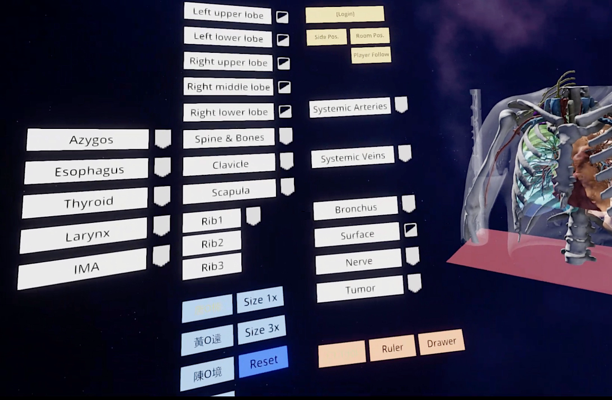
\includegraphics[width=.9\linewidth]{../Media/GUI}  
  \caption{Graphical User Interface.}
  \label{fig:GUI}
\end{figure}

A concurrent 2D slice image viewer was developed for comparison and correlation between 3D models and conventional medical images, including CT and MRI. A virtual cutting plane on the 3D models represented the corresponding level of the slice (Figure \ref{fig:CuttingPlane}) and translated accordingly when the user scrolled through the images.
\begin{figure}
  \centering
  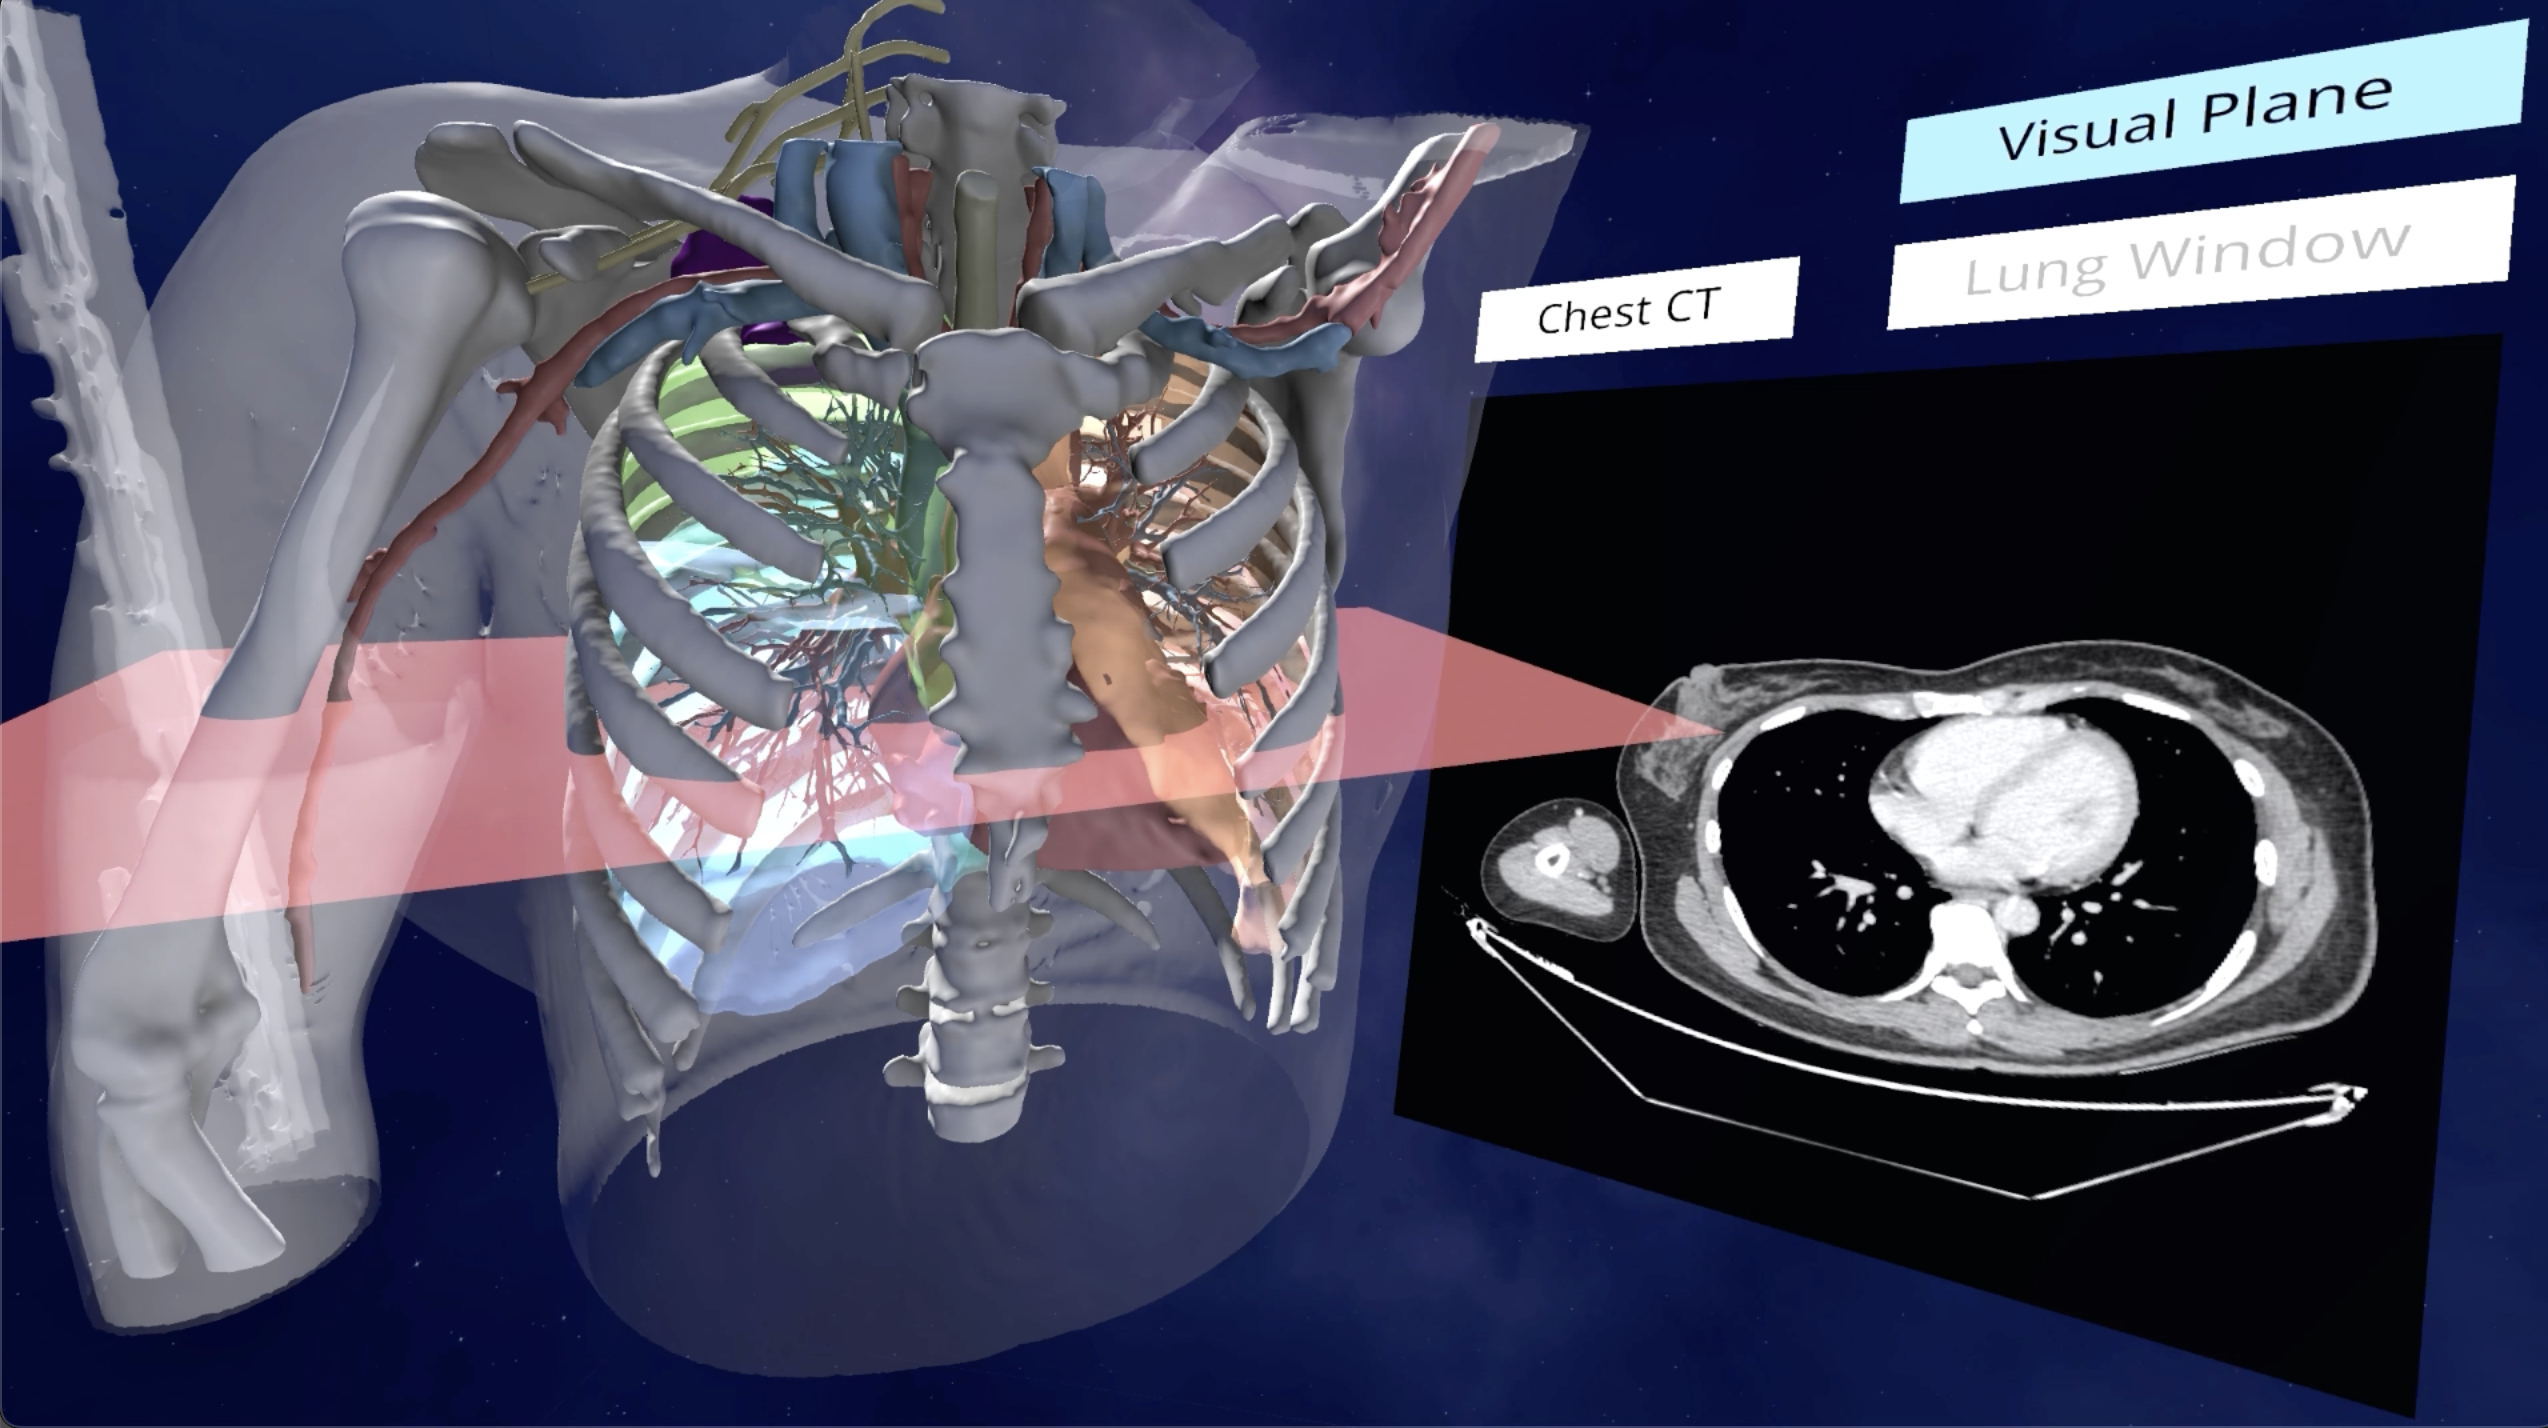
\includegraphics[width=.9\linewidth]{../Media/CuttingPlane.png}  
  \caption{Virtual cutting plane of 3D model and corresponding CT slice.}
  \label{fig:CuttingPlane}
\end{figure}
\subsection{Synchronous Sharing}
To enable real-time collaboration, education, and general communication, we develop a streaming feature that allows users without HMDs to join the preoperative planning system using conventional input devices and built-in browsers. Leveraging web real-time communication (WebRTC), we establish an extended reality (XR) cloud streaming service and a server. When the main user interacts with the system, updates are sent to the server, which then multicasts these updates to other clients \cite{RN12}. Additionally, audio from the main user can be broadcasted to remote audiences.
\section{Methods}
We design a pilot study with 10 participants, including 3 attending surgeons and 7 residents. The purpose of the study is to perform an initial validation of the system and the recorded data rather than to characterize the performance of the participants. Written informed consent is obtained from all patients included for VR collaborative surgical planning with the system described above. After an introduction and familiarization session with the system, all participating physicians evaluate the patient-specific models as the main user, with no time limitations. Each participant also joins an additional session using smartphones to participate online. This study is approved by Research Ethics Committee of our institutional review board under 202305019RINC (approval date 2023/10/23). Informed consent is obtained from all participants, including physicians and patients.

\section{Results}
The presented pipeline requires approximately an hour from importing raw data to presentation of 3D models in the VR system. This time estimate comes from running the program on the aforementioned computing resources and device. 
The segmentation and visual fidelity of the end product was verified in both conventional 2D displays and HMDs, which are rated functionally accurate by all partcipants. The results for one patient are shown in Figure \ref{fig:GUI}, \ref{fig:CuttingPlane} and video in Supplementary data. 
\section{Discussion}
Surgical interventions for complex pathologies are highly intricate, requiring precise planning to optimize outcomes while preserving critical structures. These challenges necessitate advanced preoperative planning solutions that enable detailed visualization and interaction with patient-specific anatomy. Our virtual reality collaborative preoperative planning system addresses these needs by providing a workflow for reconstructing patient-specific 3D anatomic models from 2D image data. This VR system facilitates collaborative interaction and annotation of these virtual models in an immersive environment.

The quality of the input data directly affects the fidelity of the 3D reconstructions in the virtual environment \cite{RN7, RN45}. To avoid loss of detail in the 3D models, acquisition and processing parameters of CT/MRI data need to be calibrated and standardized. Slice thickness of CT has been shown to be one of the primary factors affecting 3D model resolution and quality, with multiple studies proposing a maximum threshold of 1.25 mm \cite{RN7, RN47}. Consequently, we adopted a similar setting for input quality selection in our study.

The segmentation process is one of the most time- and resource-critical steps in generating anatomically accurate models. Manual segmentation by trained physicians or technicians has been extensively adopted in previous studies, achieving acceptable accuracy \cite{RN17, RN48, RN49}. However, the workload of manual tracing limits its efficiency, cost-effectiveness, and reproducibility. Semi-automatic or automatic segmentation aims to replace manual labor with computational processes. Methodologies including thresholding, neural networks, and other machine learning algorithms have been reported for segmenting normal tissues \cite{RN50} or pathologies \cite{RN52, RN54, RN55} across different regions. Semi-automatic segmentation alleviates the manual workload by efficiently producing segments of different organs while preserving the flexibility of manual editing for rare anatomical variations or complex pathologies. As demonstrated in our study, integrating semi-automatic segmentation into the generation of 3D-VR models has proven feasible and clinically useful for preoperative planning \cite{RN10, RN23}. A fully automatic process to segment multiple structures within a region of interest could potentially further improve efficiency and facilitate streamlining the process into an executable pipeline \cite{RN51, RN57, RN56}. However, there is still limited evidence on the feasibility of incorporating such a strategy into clinical planning \cite{RN9}.

Mesh optimization is essential in virtual reality (VR) to ensure smooth and immersive user experiences \cite{RN58}. Optimization techniques like polygon reduction and smoothing are crucial for managing the high computational demands of VR applications \cite{RN58, RN59}. Several open-source computer-aided design software packages are available and validated for generating and editing 3D medical models \cite{RN60, RN5}. In our study, we adopted MeshLab, which provides a wide range of advanced tools and functionalities and is supported by some of the largest online communities at present times \cite{RN61}.

Implementing multi-user collaboration in a virtual environment provides an innovative way for communication in medical settings. The benefits extend beyond preoperative planning into surgical simulation, personnel training, and education purposes \cite{RN64, RN26, RN65}. To maximize the advantages of collaborative features while addressing the cost of current HMDs, our system allows users to join via conventional devices with network connection and browsers. This approach not only ensures convenience and accessibility but also offers a comparable user experience for those using non-HMD devices, facilitating spectating and interaction without compromising the overall quality \cite{RN63}.


\section{Conclusion and Future Work}
We present the system architecture and technical setup of ColabSurgVR, a virtual reality collaborative system for preoperative planning. Our workflow involves creating detailed, patient-specific anatomical models from 2D image data and presenting them in an immersive, three-dimensional visualization platform. This interactive environment enhances the accuracy of surgical planning and enables real-time collaboration among multidisciplinary teams. Initial validation through a prospective pilot study with clinical participants demonstrated the system's accuracy and potential clinical benefits.
Future research will focus on enhancing the capabilities and usability of our VR system. One area of focus is optimizing computational processes to achieve rapid turnaround times suitable for emergent surgeries. Additionally, expanding and validating the VR system's application in clinical practice through comparative trials with more participants and patients will help assess its clinical impact on both surgeon-specific and patient outcomes. The proposed system could also be beneficial for a wide range of clinical applications beyond surgical planning, including physician training, student teaching, case collection, and patient communication.



%%%%%%%%%%%%%%%%%%%%%%%%%%%%%%%%%%%%%%%%%%%%%%
%%                                          %%
%% Backmatter begins here                   %%
%%                                          %%
%%%%%%%%%%%%%%%%%%%%%%%%%%%%%%%%%%%%%%%%%%%%%%

\begin{backmatter}

% \section*{Abbreviations}%% if any
% Text for this section\ldots

\section*{Acknowledgements}%% if any
We thank the patients who participated in this study, as well as all the research staff for their dedication to the research process.

\section*{Funding}%% if any
This work has been supported by National Taiwan University Hospital (113-M0029).

% \section*{Availability of data and materials}%% if any
% Text for this section\ldots

\section*{Ethics approval and consent to participate}%% if any
This study received approval from the Institutional Review Board of National Taiwan University Hospital Research Ethics Committee approved the study (project approval number 202305019RINC). The research was carried out in accordance with the Declaration 
of Helsinki.

\section*{Competing interests}
The authors declare that they have no competing interests.

% \section*{Consent for publication}%% if any
% Text for this section\ldots

% \section*{Authors' contributions}


% \section*{Authors' information}%% if any
% Text for this section\ldots

%%%%%%%%%%%%%%%%%%%%%%%%%%%%%%%%%%%%%%%%%%%%%%%%%%%%%%%%%%%%%
%%                  The Bibliography                       %%
%%                                                         %%
%%  Bmc_mathpys.bst  will be used to                       %%
%%  create a .BBL file for submission.                     %%
%%  After submission of the .TEX file,                     %%
%%  you will be prompted to submit your .BBL file.         %%
%%                                                         %%
%%                                                         %%
%%  Note that the displayed Bibliography will not          %%
%%  necessarily be rendered by Latex exactly as specified  %%
%%  in the online Instructions for Authors.                %%
%%                                                         %%
%%%%%%%%%%%%%%%%%%%%%%%%%%%%%%%%%%%%%%%%%%%%%%%%%%%%%%%%%%%%%

% if your bibliography is in bibtex format, use those commands:
\bibliographystyle{bmc-mathphys} % Style BST file (bmc-mathphys, vancouver, spbasic).
\bibliography{bmc_article}      % Bibliography file (usually '*.bib' )
% for author-year bibliography (bmc-mathphys or spbasic)
% a) write to bib file (bmc-mathphys only)
% @settings{label, options="nameyear"}
% b) uncomment next line
%\nocite{label}

% or include bibliography directly:
% \begin{thebibliography}
% \bibitem{b1}
% \end{thebibliography}

%%%%%%%%%%%%%%%%%%%%%%%%%%%%%%%%%%%
%%                               %%
%% Figures                       %%
%%                               %%
%% NB: this is for captions and  %%
%% Titles. All graphics must be  %%
%% submitted separately and NOT  %%
%% included in the Tex document  %%
%%                               %%
%%%%%%%%%%%%%%%%%%%%%%%%%%%%%%%%%%%

%%
%% Do not use \listoffigures as most will included as separate files

% \section*{Figures}
%   \begin{figure}[h!]
%   \caption{Sample figure title}
% \end{figure}

% \begin{figure}[h!]
%   \caption{Sample figure title}
% \end{figure}

%%%%%%%%%%%%%%%%%%%%%%%%%%%%%%%%%%%
%%                               %%
%% Tables                        %%
%%                               %%
%%%%%%%%%%%%%%%%%%%%%%%%%%%%%%%%%%%

%% Use of \listoftables is discouraged.
%%
% \section*{Tables}
% \begin{table}[h!]
% \caption{Sample table title. This is where the description of the table should go}
%   \begin{tabular}{cccc}
%     \hline
%     & B1  &B2   & B3\\ \hline
%     A1 & 0.1 & 0.2 & 0.3\\
%     A2 & ... & ..  & .\\
%     A3 & ..  & .   & .\\ \hline
%   \end{tabular}
% \end{table}

%%%%%%%%%%%%%%%%%%%%%%%%%%%%%%%%%%%
%%                               %%
%% Additional Files              %%
%%                               %%
%%%%%%%%%%%%%%%%%%%%%%%%%%%%%%%%%%%

% \section*{Additional Files}
%   \subsection*{Additional file 1 --- Sample additional file title}
%     Additional file descriptions text (including details of how to
%     view the file, if it is in a non-standard format or the file extension).  This might
%     refer to a multi-page table or a figure.

%   \subsection*{Additional file 2 --- Sample additional file title}
%     Additional file descriptions text.





\end{backmatter}
\end{document}
